\documentclass[10pt,aspectratio=169]{beamer}
\usepackage[utf8]{inputenc}
\usepackage{listings}
\usepackage{hyperref}
\usepackage{xcolor}
\usepackage{ragged2e}
\usepackage{graphicx}
\usepackage{tikz}
\usetikzlibrary{positioning,calc,decorations.pathreplacing}

\usetheme{Dresden}
%\usetheme{Bergen}

\title{Programming Techniques 2026--2027}
\author{Hannu Parviainen}
\institute{Universidad de la Laguna}
\date{\today}

% Single spaces after full stops, so that e.g. \texttt{a .dot. b} has even spacing
\frenchspacing

\lstset{
  language=fortran,
  basicstyle=\ttfamily\scriptsize,
  columns=fullflexible,
  keepspaces=true,
  backgroundcolor=\color{white},
  keywordstyle=\color{blue},
  commentstyle=\color{gray},
  stringstyle=\color{red},
  showstringspaces=false,
  breaklines=true,
  frame=lines
}

\subtitle{Lecture 9: Shared-Memory Parallelisation with OpenMP}

\begin{document}

\begin{frame}
  \titlepage
\end{frame}


\section{Introduction}

\begin{frame}
  \centering
  \Huge \textbf{Introduction to OpenMP}
\end{frame}


\begin{frame}
  \frametitle{What is OpenMP?}
  \begin{columns}[T]
    \begin{column}{0.5\textwidth}
      \begin{itemize}
        \item OpenMP (Open Multi-Processing) is a portable programming interface for \emph{shared-memory} parallel computing.
        \item It is a standard for Fortran and C/C++, and works on Linux, Windows, and macOS.
        \item It needs a compiler that supports OpenMP. Most modern compilers do, including \texttt{gfortran}.
        \item The first specification for Fortran came out in 1997. Version 6.0 was released in November 2024.
      \end{itemize}
    \end{column}

    \begin{column}{0.5\textwidth}
      \begin{itemize}
        \item OpenMP is built around a \emph{fork--join} model: one thread runs the program and starts a team of threads where there is parallel work.
        \item A serial program can be parallelised in small steps, one loop at a time. There is no need to rewrite it from scratch.
        \item The serial and parallel versions of a program can live in the same source code.
      \end{itemize}
    \end{column}
  \end{columns}
\end{frame}


\begin{frame}
  \frametitle{Shared and distributed memory}
  \begin{columns}[T]
    \begin{column}{0.5\textwidth}
      \centering
      \textbf{Shared memory: OpenMP}

      \vspace*{3mm}
      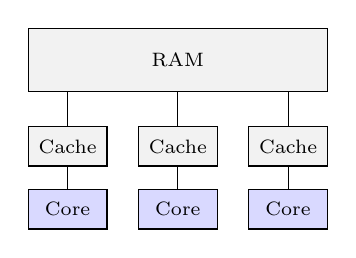
\begin{tikzpicture}[box/.style={draw, fill=gray!10, minimum height=5mm, minimum width=10mm, font=\scriptsize}]
        \node[box, minimum width=38mm, minimum height=8mm] (ram) at (0,1.8) {RAM};
        \foreach \k/\x in {1/-1.4, 2/0, 3/1.4} {
          \node[box] (c\k) at (\x,0.7) {Cache};
          \node[box, fill=blue!15] (p\k) at (\x,-0.1) {Core};
          \draw (p\k) -- (c\k) -- (c\k |- ram.south);
        }
      \end{tikzpicture}

      \vspace*{3mm}
      \raggedright
      All the cores of one computer read and write the same memory. The threads of a program see the same variables.
    \end{column}

    \begin{column}{0.5\textwidth}
      \centering
      \textbf{Distributed memory: MPI}

      \vspace*{3mm}
      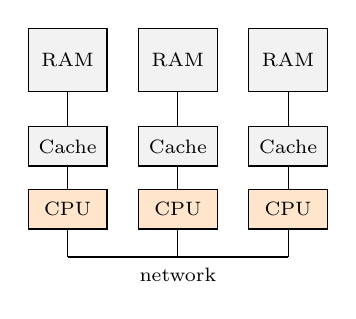
\begin{tikzpicture}[box/.style={draw, fill=gray!10, minimum height=5mm, minimum width=10mm, font=\scriptsize}]
        \foreach \k/\x in {1/-1.4, 2/0, 3/1.4} {
          \node[box, minimum height=8mm] (m\k) at (\x,1.8) {RAM};
          \node[box] (c\k) at (\x,0.7) {Cache};
          \node[box, fill=orange!20] (p\k) at (\x,-0.1) {CPU};
          \draw (p\k) -- (c\k) -- (m\k);
          \draw (p\k.south) -- ++(0,-0.35);
        }
        \draw[thick] (-1.4,-0.71) -- node[below, font=\scriptsize] {network} (1.4,-0.71);
      \end{tikzpicture}

      \vspace*{-1mm}
      \raggedright
      Each processor has its own memory. The processes exchange data by sending messages over a network.
    \end{column}
  \end{columns}
\end{frame}


\begin{frame}
  \frametitle{OpenMP, MPI, or both?}
  \begin{columns}[T]
    \begin{column}{0.5\textwidth}
      \textbf{OpenMP}
      \begin{itemize}
        \item runs on one shared-memory computer,
        \item parallelises a serial program step by step, in the same source,
        \item and leaves much of the work to the compiler.
      \end{itemize}

      \textbf{MPI}
      \begin{itemize}
        \item runs on shared- and distributed-memory systems,
        \item needs a program designed for it, and an MPI library,
        \item and leaves more of the work to the programmer.
      \end{itemize}
    \end{column}

    \begin{column}{0.5\textwidth}
      \centering
      \textbf{Hybrid: MPI between nodes, OpenMP inside them}

      \vspace*{3mm}
      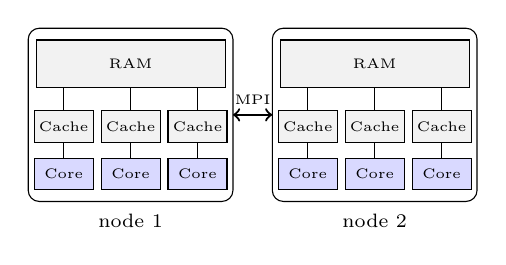
\begin{tikzpicture}[box/.style={draw, fill=gray!10, minimum height=4mm, minimum width=7.5mm, inner sep=1pt, font=\tiny}]
        \foreach \n/\cx in {1/-1.55, 2/1.55} {
          \node[box, minimum width=24mm, minimum height=6mm] (ram\n) at (\cx,1.4) {RAM};
          \foreach \k/\dx in {1/-0.85, 2/0, 3/0.85} {
            \node[box] (c\n\k) at (\cx+\dx,0.6) {Cache};
            \node[box, fill=blue!15] (p\n\k) at (\cx+\dx,0) {Core};
            \draw (p\n\k) -- (c\n\k) -- (c\n\k |- ram\n.south);
          }
          \draw[rounded corners] (\cx-1.3,-0.35) rectangle (\cx+1.3,1.85);
          \node[font=\scriptsize] at (\cx,-0.6) {node \n};
        }
        \draw[thick, <->] (-0.25,0.75) -- node[above, font=\tiny] {MPI} (0.25,0.75);
      \end{tikzpicture}

      \vspace*{3mm}
      \raggedright
      Large clusters combine the two: one MPI process per node, and OpenMP threads on the cores of that node.
    \end{column}
  \end{columns}
\end{frame}


\begin{frame}[fragile]
  \frametitle{Directives}
  \begin{columns}[T]
    \begin{column}{0.55\textwidth}
      \begin{itemize}
        \item OpenMP is mostly written as \emph{directives}. They tell the compiler how to share the work between threads. \emph{Clauses} modify the directives.
        \item A directive is a comment that starts with the \emph{sentinel} \texttt{!\$omp}.
        \item A long directive is continued with \texttt{\&}, and the next line starts again with \texttt{!\$omp}.
        \item A compiler without OpenMP, or without the \texttt{-fopenmp} flag, sees the directives as ordinary comments and ignores them.
        \item So the same source compiles to a serial or a parallel program.
      \end{itemize}
    \end{column}

    \begin{column}{0.45\textwidth}
      \begin{lstlisting}
!$omp directive [clause, clause, ...]
...
!$omp end directive
      \end{lstlisting}

      \vspace*{2mm}
      A directive split over three lines:
      \begin{lstlisting}
!$omp parallel do private(x, y) &
!$omp shared(a, b) &
!$omp reduction(+:total)
      \end{lstlisting}

      \vspace*{2mm}
      Compiling with and without OpenMP:
      \begin{lstlisting}[language=bash]
gfortran -fopenmp -o prog prog.f90
gfortran -o prog prog.f90
      \end{lstlisting}
    \end{column}
  \end{columns}
\end{frame}


\section{Parallel regions}

\begin{frame}
  \centering
  \Huge \textbf{Parallel Regions}
\end{frame}


\begin{frame}[fragile]
  \frametitle{A parallel region}
  \begin{columns}[T]
    \begin{column}{0.36\textwidth}
      \begin{itemize}
        \item The \texttt{parallel} directive starts a team of threads.
        \item Every thread runs the code between \texttt{!\$omp parallel} and \texttt{!\$omp end parallel}.
        \item By default, there is one thread per logical core. Here, the environment variable \texttt{OMP\_NUM\_THREADS} sets the number to four.
      \end{itemize}
    \end{column}

    \begin{column}{0.32\textwidth}
      \begin{lstlisting}
program hello_omp
  implicit none

  print *, 'Before parallel'

  !$omp parallel
  print *, 'Inside parallel'
  !$omp end parallel

  print *, 'After parallel'
end program hello_omp
      \end{lstlisting}
    \end{column}

    \begin{column}{0.32\textwidth}
      Compiled without \texttt{-fopenmp}:
      \begin{lstlisting}[language=bash]
$ ./hello_omp
 Before parallel
 Inside parallel
 After parallel
      \end{lstlisting}

      \vspace*{1mm}
      Compiled with \texttt{-fopenmp}:
      \begin{lstlisting}[language=bash]
$ OMP_NUM_THREADS=4 ./hello_omp
 Before parallel
 Inside parallel
 Inside parallel
 Inside parallel
 Inside parallel
 After parallel
      \end{lstlisting}
    \end{column}
  \end{columns}
\end{frame}


\begin{frame}
  \frametitle{The fork--join model}
  \begin{columns}[T]
    \begin{column}{0.42\textwidth}
      \begin{itemize}
        \item The program starts with one thread, the \emph{master} thread (thread 0).
        \item At \texttt{!\$omp parallel}, it \emph{forks} a team of threads. The master thread is part of the team.
        \item At \texttt{!\$omp end parallel}, the threads \emph{join}: the master waits until all the threads have finished, and then continues alone.
        \item Starting and stopping a team costs time, so a parallel region should contain enough work.
      \end{itemize}
    \end{column}

    \begin{column}{0.58\textwidth}
      \centering
      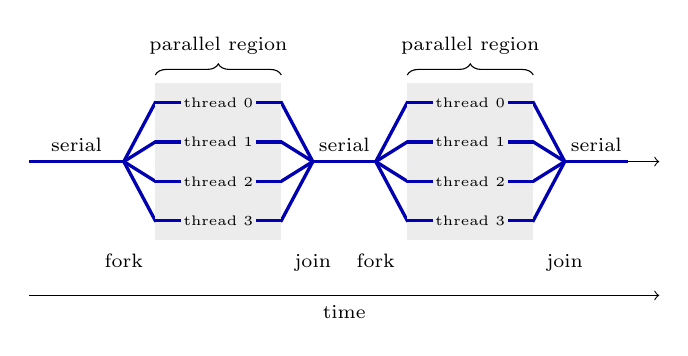
\begin{tikzpicture}[x=1cm, y=1cm, thread/.style={very thick, blue!70!black}]
        % serial parts
        \draw[thread] (0,0) -- (1.2,0);
        \draw[thread] (3.6,0) -- (4.4,0);
        \draw[thread] (6.8,0) -- (7.6,0);
        % parallel regions
        \foreach \s in {1.2, 4.4} {
          \foreach \y in {0.75, 0.25, -0.25, -0.75} {
            \draw[thread] (\s,0) -- (\s+0.4,\y) -- (\s+2.0,\y) -- (\s+2.4,0);
          }
          \fill[gray!15] (\s+0.4,-1.0) rectangle (\s+2.0,1.0);
          \foreach \y/\t in {0.75/0, 0.25/1, -0.25/2, -0.75/3} {
            \draw[thread] (\s+0.4,\y) -- (\s+2.0,\y);
            \node[font=\tiny, fill=gray!15, inner sep=1pt] at (\s+1.2,\y) {thread \t};
          }
        }
        \draw[->] (7.6,0) -- (8.0,0);
        % labels
        \node[font=\scriptsize, above] at (0.6,0) {serial};
        \node[font=\scriptsize, above] at (4.0,0) {serial};
        \node[font=\scriptsize, above] at (7.2,0) {serial};
        \node[font=\scriptsize, below] at (1.2,-1.05) {fork};
        \node[font=\scriptsize, below] at (3.6,-1.05) {join};
        \node[font=\scriptsize, below] at (4.4,-1.05) {fork};
        \node[font=\scriptsize, below] at (6.8,-1.05) {join};
        \draw[decorate, decoration={brace, amplitude=4pt}] (1.6,1.1) -- node[above=4pt, font=\scriptsize] {parallel region} (3.2,1.1);
        \draw[decorate, decoration={brace, amplitude=4pt}] (4.8,1.1) -- node[above=4pt, font=\scriptsize] {parallel region} (6.4,1.1);
        \draw[->] (0,-1.7) -- node[below, font=\scriptsize] {time} (8.0,-1.7);
      \end{tikzpicture}
    \end{column}
  \end{columns}
\end{frame}


\begin{frame}[fragile]
  \frametitle{Thread numbers: the \texttt{omp\_lib} module}
  \begin{columns}[T]
    \begin{column}{0.45\textwidth}
      \begin{itemize}
        \item The \texttt{omp\_lib} module has procedures that query and control the threads:
          \begin{itemize}
            \item \texttt{omp\_get\_num\_threads()}: the number of threads in the team,
            \item \texttt{omp\_get\_thread\_num()}: the number of this thread, from 0 to $n-1$,
            \item \texttt{omp\_get\_wtime()}: the wall-clock time in seconds.
          \end{itemize}
        \item Each thread needs its own \texttt{n\_threads} and \texttt{id}, so they are \texttt{private}. More about this later.
        \item The threads run at the same time, so the order of the output changes from run to run.
      \end{itemize}
    \end{column}

    \begin{column}{0.55\textwidth}
      \begin{lstlisting}
program thread_ids
  use omp_lib
  implicit none
  integer :: n_threads, id

  !$omp parallel private(n_threads, id)
  n_threads = omp_get_num_threads()
  id = omp_get_thread_num()
  print '(a, i0, a, i0)', 'Thread ', id, ' of ', n_threads
  !$omp end parallel
end program thread_ids
      \end{lstlisting}

      \begin{lstlisting}[language=bash]
$ gfortran -fopenmp -o thread_ids thread_ids.f90
$ OMP_NUM_THREADS=4 ./thread_ids
Thread 2 of 4
Thread 1 of 4
Thread 3 of 4
Thread 0 of 4
      \end{lstlisting}
    \end{column}
  \end{columns}
\end{frame}


\begin{frame}[fragile]
  \frametitle{Compiling without OpenMP}
  \begin{itemize}
    \item The directives are ignored without \texttt{-fopenmp}, but the calls to \texttt{omp\_lib} are ordinary Fortran. Compiling \texttt{thread\_ids.f90} without OpenMP fails:
  \end{itemize}

  \begin{lstlisting}[language=bash]
$ gfortran -o thread_ids thread_ids.f90
/usr/bin/ld: /tmp/ccM4ag4r.o: in function `MAIN__':
thread_ids.f90:(.text+0xc): undefined reference to `omp_get_num_threads_'
/usr/bin/ld: thread_ids.f90:(.text+0x14): undefined reference to `omp_get_thread_num_'
collect2: error: ld returned 1 exit status
  \end{lstlisting}

  \begin{itemize}
    \item The compiler finds the module, but the linker does not link the OpenMP runtime library that contains the procedures.
    \item The same happens with a compiler that does not support OpenMP. We would lose one of the main advantages of OpenMP: one source for both the serial and the parallel program.
  \end{itemize}
\end{frame}


\begin{frame}[fragile]
  \frametitle{Conditional compilation}
  \begin{columns}[T]
    \begin{column}{0.45\textwidth}
      \begin{itemize}
        \item A line that starts with the sentinel \texttt{!\$} followed by a space is compiled only with OpenMP. Otherwise, it is a comment.
        \item Use it for \texttt{use omp\_lib} and for every call to an OpenMP procedure.
        \item The serial program gets the default values: one thread, number 0.
        \item Private variables start \emph{undefined} in each thread, so the default values are set inside the parallel region.
      \end{itemize}
    \end{column}

    \begin{column}{0.55\textwidth}
      \begin{lstlisting}
program thread_ids_portable
  !$ use omp_lib
  implicit none
  integer :: n_threads, id

  !$omp parallel private(n_threads, id)
  n_threads = 1
  id = 0
  !$ n_threads = omp_get_num_threads()
  !$ id = omp_get_thread_num()
  print '(a, i0, a, i0)', 'Thread ', id, ' of ', n_threads
  !$omp end parallel
end program thread_ids_portable
      \end{lstlisting}

      \begin{lstlisting}[language=bash]
$ gfortran -o thread_ids_portable thread_ids_portable.f90
$ ./thread_ids_portable
Thread 0 of 1
      \end{lstlisting}
    \end{column}
  \end{columns}
\end{frame}


\begin{frame}[fragile]
  \frametitle{Setting the number of threads}
  \begin{columns}[T]
    \begin{column}{0.55\textwidth}
      There are three ways, from the weakest to the strongest:
      \begin{enumerate}
        \item the environment variable \texttt{OMP\_NUM\_THREADS} sets the default for the whole program,
        \item \texttt{omp\_set\_num\_threads(n)} sets it for the following parallel regions, and
        \item the \texttt{num\_threads(n)} clause sets it for one region.
      \end{enumerate}

      \vspace*{2mm}
      \begin{itemize}
        \item Without any of them, there is one thread per logical core.
        \item \texttt{omp\_get\_max\_threads()} returns the size of the next team. Outside a parallel region, \texttt{omp\_get\_num\_threads()} returns 1.
      \end{itemize}
    \end{column}

    \begin{column}{0.45\textwidth}
      \begin{lstlisting}[language=bash]
$ export OMP_NUM_THREADS=4   # this shell
$ ./prog
$ OMP_NUM_THREADS=2 ./prog   # one run
      \end{lstlisting}

      \vspace*{2mm}
      \begin{lstlisting}
!$ call omp_set_num_threads(4)

!$omp parallel num_threads(2)
...
!$omp end parallel
      \end{lstlisting}
    \end{column}
  \end{columns}
\end{frame}


\section{Loops}

\begin{frame}
  \centering
  \Huge \textbf{Parallel Loops}
\end{frame}


\begin{frame}[fragile]
  \frametitle{Sharing the work of a loop}
  \begin{columns}[T]
    \begin{column}{0.45\textwidth}
      \begin{itemize}
        \item Having every thread repeat the same work is pointless. A \emph{worksharing} construct divides the work between the threads.
        \item \texttt{!\$omp do} divides the iterations of the next \texttt{do} loop between the threads of the team. Each iteration is run by exactly one thread.
        \item \texttt{!\$omp do} must be inside a parallel region. Otherwise, the team has one thread.
        \item The array \texttt{a} is shared. Each thread writes different elements of it.
      \end{itemize}
    \end{column}

    \begin{column}{0.55\textwidth}
      \begin{lstlisting}
program parallel_loop
  !$ use omp_lib
  implicit none
  integer, parameter :: n = 8
  real :: a(n)
  integer :: i, id

  !$omp parallel private(i, id) shared(a)
  id = 0
  !$ id = omp_get_thread_num()
  !$omp do
  do i = 1, n
    a(i) = i**2 + 3.0
    print '(a, i0, a, i0)', 'i = ', i, ' on thread ', id
  end do
  !$omp end do
  !$omp end parallel
  print '(*(f6.1))', a
end program parallel_loop
      \end{lstlisting}
    \end{column}
  \end{columns}
\end{frame}


\begin{frame}[fragile]
  \frametitle{Sharing the work of a loop: the output}
  \begin{columns}[T]
    \begin{column}{0.25\textwidth}
      Without OpenMP:
      \begin{lstlisting}[language=bash]
i = 1 on thread 0
i = 2 on thread 0
i = 3 on thread 0
i = 4 on thread 0
i = 5 on thread 0
i = 6 on thread 0
i = 7 on thread 0
i = 8 on thread 0
      \end{lstlisting}
    \end{column}

    \begin{column}{0.25\textwidth}
      Four threads:
      \begin{lstlisting}[language=bash]
i = 1 on thread 0
i = 2 on thread 0
i = 5 on thread 2
i = 6 on thread 2
i = 7 on thread 3
i = 8 on thread 3
i = 3 on thread 1
i = 4 on thread 1
      \end{lstlisting}
    \end{column}

    \begin{column}{0.5\textwidth}
      \begin{itemize}
        \item By default, each thread gets one contiguous block of iterations:
      \end{itemize}

      \vspace*{2mm}
      \centering
      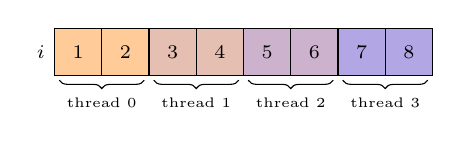
\begin{tikzpicture}[x=6mm, y=6mm]
        \foreach \i in {1,...,8} {
          \pgfmathtruncatemacro{\t}{(\i-1)/2}
          \pgfmathsetmacro{\c}{\t*25}
          \fill[blue!\c!orange!40] (\i-1,0) rectangle (\i,1);
          \draw (\i-1,0) rectangle (\i,1);
          \node[font=\scriptsize] at (\i-0.5,0.5) {\i};
        }
        \foreach \t in {0,...,3} {
          \draw[decorate, decoration={brace, amplitude=3pt, mirror}] (2*\t+0.1,-0.1) -- node[below=3pt, font=\tiny] {thread \t} (2*\t+1.9,-0.1);
        }
        \node[font=\scriptsize, left] at (0,0.5) {$i$};
      \end{tikzpicture}

      \raggedright
      \begin{itemize}
        \item The threads run at the same time, so the lines are printed in a different order every run.
        \item The array is the same in both cases:
      \end{itemize}
      \begin{lstlisting}[language=bash]
   4.0   7.0  12.0  19.0  28.0  39.0  52.0  67.0
      \end{lstlisting}
    \end{column}
  \end{columns}
\end{frame}


\begin{frame}[fragile]
  \frametitle{The combined \texttt{parallel do}}
  \begin{columns}[T]
    \begin{column}{0.5\textwidth}
      \begin{itemize}
        \item A parallel region that contains only one loop can be written with one combined directive.
        \item The clauses of both directives can be given to the combined one.
        \item The loop index is private automatically.
        \item There is an implicit \emph{barrier} at \texttt{end do}: the threads wait for each other before they continue.
        \item The number of iterations must be known when the loop starts. A \texttt{do while} loop, or a loop with \texttt{exit}, cannot be shared.
      \end{itemize}
    \end{column}

    \begin{column}{0.5\textwidth}
      \begin{lstlisting}
!$omp parallel
!$omp do
do i = 1, n
  a(i) = i**2 + 3.0
end do
!$omp end do
!$omp end parallel
      \end{lstlisting}

      \vspace*{2mm}
      is the same as
      \begin{lstlisting}
!$omp parallel do
do i = 1, n
  a(i) = i**2 + 3.0
end do
!$omp end parallel do
      \end{lstlisting}
    \end{column}
  \end{columns}
\end{frame}


\begin{frame}[fragile]
  \frametitle{Which loops can be parallelised?}
  \begin{columns}[T]
    \begin{column}{0.45\textwidth}
      \begin{itemize}
        \item The iterations must be \emph{independent}: they must give the same result when they run in any order, or at the same time.
        \item OpenMP does not check this. It does what the directive says, also when the result is wrong.
        \item A loop where each iteration needs the result of the previous one has to be rewritten, or left serial.
      \end{itemize}
    \end{column}

    \begin{column}{0.55\textwidth}
      \begin{lstlisting}
! Independent iterations: can be parallelised.
do i = 1, n
  c(i) = a(i) + b(i)
end do

! Each iteration needs the result of the previous
! one: cannot be parallelised as it is.
do i = 2, n
  a(i) = a(i-1) + b(i)
end do

! Every iteration updates the same variable:
! needs a reduction (later today).
do i = 1, n
  total = total + a(i)
end do
      \end{lstlisting}
    \end{column}
  \end{columns}
\end{frame}


\begin{frame}[fragile]
  \frametitle{Nested loops and \texttt{collapse}}
  \begin{columns}[T]
    \begin{column}{0.4\textwidth}
      \begin{itemize}
        \item \texttt{!\$omp do} shares only the outer loop. Here, with four threads, one thread would be idle.
        \item \texttt{collapse(2)} shares all the $4 \times 3 = 12$ iterations.
        \item The loops must be perfectly nested.
      \end{itemize}

      \vspace*{1mm}
      Four threads:
      \begin{columns}[T]
        \begin{column}{0.5\textwidth}
          \begin{lstlisting}[language=bash]
(1,1) on thread 0
(2,1) on thread 0
(3,1) on thread 0
(4,1) on thread 1
(1,2) on thread 1
(2,2) on thread 1
          \end{lstlisting}
        \end{column}
        \begin{column}{0.5\textwidth}
          \begin{lstlisting}[language=bash]
(2,3) on thread 3
(3,3) on thread 3
(4,3) on thread 3
(3,2) on thread 2
(4,2) on thread 2
(1,3) on thread 2
          \end{lstlisting}
        \end{column}
      \end{columns}
    \end{column}

    \begin{column}{0.6\textwidth}
      \begin{lstlisting}
program collapse
  !$ use omp_lib
  implicit none
  real :: a(4,3)
  integer :: i, j, id

  !$omp parallel private(i, j, id) shared(a)
  id = 0
  !$ id = omp_get_thread_num()
  !$omp do collapse(2)
  do j = 1, 3
    do i = 1, 4
      a(i,j) = i + j
      print '(3(a, i0))', '(', i, ',', j, ') on thread ', id
    end do
  end do
  !$omp end do
  !$omp end parallel
end program collapse
      \end{lstlisting}
    \end{column}
  \end{columns}
\end{frame}


\section{Data sharing}

\begin{frame}
  \centering
  \Huge \textbf{Shared and Private Data}
\end{frame}


\begin{frame}[fragile]
  \frametitle{Shared and private variables}
  \begin{columns}[T]
    \begin{column}{0.55\textwidth}
      \begin{itemize}
        \item A \texttt{shared} variable exists once, and all the threads use the same memory.
        \item A \texttt{private} variable has a separate copy in each thread. The copies start \emph{undefined}, and are lost at the end of the region.
        \item \texttt{firstprivate}: private, but each copy starts with the value from before the region.
        \item \texttt{lastprivate} (on \texttt{do}): private, and the value from the last iteration is copied out after the loop.
        \item By default, variables are shared, except the indices of parallel loops.
        \item \texttt{default(none)} turns the defaults off, so the compiler catches forgotten variables.
      \end{itemize}
    \end{column}

    \begin{column}{0.45\textwidth}
      \begin{lstlisting}
!$omp parallel do default(none) &
!$omp shared(a, b, c, n) private(x, y)
do i = 1, n
  x = a(i) + b(i)
  y = a(i) - b(i)
  c(i) = x * y
end do
!$omp end parallel do
      \end{lstlisting}

      \vspace*{1mm}
      \begin{block}{Rules of thumb}
        \small
        Only read, or each thread writes its own elements: \texttt{shared}. A temporary value in an iteration: \texttt{private}. Updated by every iteration: \texttt{reduction}.
      \end{block}
    \end{column}
  \end{columns}
\end{frame}


\begin{frame}[fragile]
  \frametitle{Race conditions}
  \begin{columns}[T]
    \begin{column}{0.44\textwidth}
      \begin{itemize}
        \item A \emph{race condition} happens when two threads access the same variable at the same time, and at least one of them writes to it.
        \item \texttt{total = total + 1} is three steps: read, add one, and write back. Two threads can read the same old value, and one addition is lost.
        \item The result is wrong, and different every run, without a crash or a warning. A program that gives the right answer once is not necessarily correct.
      \end{itemize}
    \end{column}

    \begin{column}{0.56\textwidth}
      \begin{lstlisting}
program race
  implicit none
  integer, parameter :: n = 1000000
  integer :: i, total

  total = 0
  !$omp parallel do shared(total)
  do i = 1, n
    total = total + 1
  end do
  !$omp end parallel do
  print '(2(a, i0))', 'total = ', total, ', expected ', n
end program race
      \end{lstlisting}

      \begin{lstlisting}[language=bash]
$ OMP_NUM_THREADS=4 ./race
total = 258804, expected 1000000
$ OMP_NUM_THREADS=4 ./race
total = 276099, expected 1000000
      \end{lstlisting}
    \end{column}
  \end{columns}
\end{frame}


\begin{frame}[fragile]
  \frametitle{Reductions}
  \begin{columns}[T]
    \begin{column}{0.5\textwidth}
      \begin{itemize}
        \item A \emph{reduction} combines many values into one: a sum, a product, a maximum\ldots
        \item \texttt{reduction(op:list)} gives each thread a private copy of the variables, starting from the identity of \texttt{op} (0 for \texttt{+}, 1 for \texttt{*}). At the end, the copies are combined with \texttt{op} and the original value.
        \item \texttt{reduction(+:total)} fixes the race on the previous slide.
        \item The order of the additions changes, so a floating-point result can differ from the serial one in the last digits.
      \end{itemize}

      \vspace*{1mm}
      \footnotesize
      \begin{tabular}{ll}
        Operators:  & \texttt{+  *  -  .and.  .or.  .eqv.  .neqv.} \\
        Intrinsics: & \texttt{max  min  iand  ior  ieor} \\
      \end{tabular}

    \end{column}

    \begin{column}{0.5\textwidth}
      \begin{lstlisting}
program reduction
  implicit none
  real :: a(5), b(5), dot
  integer :: i
  a = [0.1, 3.4, 7.4, 1.2, 8.3]
  b = [3.8, 0.1, 1.6, 0.1, 0.3]

  dot = 0.0
  !$omp parallel do reduction(+:dot)
  do i = 1, size(a)
    dot = dot + a(i) * b(i)
  end do
  !$omp end parallel do
  print '(a, f0.3)', 'a . b = ', dot
end program reduction
      \end{lstlisting}

      \begin{lstlisting}[language=bash]
$ OMP_NUM_THREADS=4 ./reduction
a . b = 15.170
      \end{lstlisting}
    \end{column}
  \end{columns}
\end{frame}


\begin{frame}[fragile]
  \frametitle{Summary: clauses for parallel loops}
  \centering
  \small
  \begin{tabular}{ll}
    \textbf{Clause} & \textbf{Meaning} \\
    \hline
    \texttt{shared(list)}             & one copy, used by all the threads \\
    \texttt{private(list)}            & one undefined copy per thread \\
    \texttt{firstprivate(list)}       & one copy per thread, starting with the value from before the region \\
    \texttt{lastprivate(list)}        & private, with the value of the last iteration copied out \\
    \texttt{default(none)}            & no defaults: every variable must be listed \\
    \texttt{reduction(op:list)}       & private copies, combined with \texttt{op} at the end \\
    \texttt{collapse(n)}              & share the iterations of $n$ nested loops \\
    \texttt{schedule(kind[, chunk])}  & how the iterations are divided between the threads (Lecture 10) \\
    \texttt{nowait}                   & on \texttt{end do}: no barrier at the end of the loop (Lecture 10) \\
    \texttt{num\_threads(n)}          & on \texttt{parallel}: the size of the team \\
    \hline
  \end{tabular}

  \vspace*{5mm}
  \raggedright
  \normalsize
  The force loop of course exercise 1 is a nested loop over the pairs of particles. Think about which variables are shared, which are private, and which are updated by many iterations.
\end{frame}


\section{Timing}

\begin{frame}[fragile]
  \frametitle{Measuring time and speedup}
  \begin{columns}[T]
    \begin{column}{0.5\textwidth}
      \begin{itemize}
        \item \texttt{omp\_get\_wtime()} returns the wall-clock time in seconds as a \texttt{real64}. Use the difference of two calls.
        \item Do not use \texttt{cpu\_time} for parallel code: it adds up the time of all the threads.
        \item The \emph{speedup} on $p$ threads is
          \[ S(p) = \frac{T(1)}{T(p)}, \]
          and the \emph{parallel efficiency} is $E(p) = S(p)/p$.
        \item Time the same optimised build (e.g. \texttt{-O2}), repeat the runs, and do not print inside the timed part.
      \end{itemize}
    \end{column}

    \begin{column}{0.5\textwidth}
      \begin{lstlisting}
use omp_lib
use iso_fortran_env, only: real64
real(real64) :: t0, t1

t0 = omp_get_wtime()
!$omp parallel do
do i = 1, n
  b(i) = sin(a(i)) + 2*a(i)
end do
!$omp end parallel do
t1 = omp_get_wtime()

print '(a, f6.3, a)', 'Time: ', t1 - t0, ' s'
      \end{lstlisting}

      \begin{lstlisting}[language=bash]
$ OMP_NUM_THREADS=1 ./prog
$ OMP_NUM_THREADS=4 ./prog
      \end{lstlisting}
    \end{column}
  \end{columns}
\end{frame}


\section{Exercises}

\begin{frame}{Exercise 1: parallel matrix product}
  \begin{block}{Tasks}
    \begin{enumerate}
      \item Write a subroutine that computes the matrix product $C = AB$ of two $n \times n$ matrices with three nested loops, as in the matrix product exercise of Lecture 3.
      \item Write a second version, parallelised with OpenMP so that different threads compute different columns of $C$. Which variables are shared and which are private? Use \texttt{default(none)}.
      \item Write a program that fills two matrices with random numbers, multiplies them with both versions and with the \texttt{matmul} intrinsic, checks that the results agree, and prints the wall time each one took. Use \texttt{omp\_get\_wtime}.
      \item Run the program with $n = 200$ and $n = 1000$, and with 1, 2, 4, and 8 threads. How much faster is the parallel version? Does the program still compile and run without \texttt{-fopenmp}?
    \end{enumerate}
  \end{block}
\end{frame}


\begin{frame}{Exercise 2: the trapezoidal rule}
  \begin{block}{Tasks}
    \begin{enumerate}
      \item Write a program that computes the integral
        \[ I = \int_0^3 x \sin x \, dx \]
        with the trapezoidal rule and $n$ intervals, using a parallel \texttt{do} loop and a reduction. Use 64-bit reals.
      \item Compare the result with the exact value $I = \sin 3 - 3 \cos 3 \approx 3.1110$. How does the error change when $n$ is doubled?
      \item Remove the \texttt{reduction} clause. What happens to the result, with one thread and with several?
    \end{enumerate}
  \end{block}
\end{frame}


\begin{frame}{Exercise 3: the Wallis product}
  \begin{block}{Tasks}
    \begin{enumerate}
      \item The Wallis product gives $\pi$ as an infinite product:
        \[ \frac{\pi}{2} = \prod_{n=1}^{\infty} \frac{4n^2}{4n^2 - 1} = \frac{2}{1} \cdot \frac{2}{3} \cdot \frac{4}{3} \cdot \frac{4}{5} \cdot \frac{6}{5} \cdot \frac{6}{7} \cdots \]
        Write a program that computes $\pi$ from the first $N$ terms with a parallel reduction.
      \item How many terms are needed to get five correct digits, 3.1415? Is the answer the same with 32-bit and 64-bit reals?
      \item Does the result depend on the number of threads? Why?
    \end{enumerate}
  \end{block}
\end{frame}

\end{document}
